\documentclass[11pt,a4paper]{article}
\usepackage[utf8]{inputenc}
\usepackage[T1]{fontenc}
\usepackage{amsmath}
\usepackage[usenames,dvipsnames,svgnames,table]{xcolor}
\usepackage[normalem]{ulem}
\usepackage[left=1.00cm, right=1.00cm, top=0.40cm, bottom=0.2cm]{geometry}
\PassOptionsToPackage{defaults=hu-min}{magyar.ldf}
\usepackage[magyar]{babel}
\usepackage{framed, fancyhdr, wasysym, graphicx, multirow, hyperref}

\begin{document}
	\renewcommand{\labelitemi}{\textbullet}
	\def\br{\\[0.1cm]}
	\thispagestyle{empty}
	\begin{center}
		\colorbox{lightgray}{{\large B1V655} \hspace{3cm} {\large Webes alkalmazások fejlesztése 2. beadandó} \hspace{5cm} \thepage}
	\end{center}
	\begin{framed}
		\begin{flushleft}
			{\large \textbf{Horváth Milán}}
			\hspace{3cm}{\large \textbf{2.Beadandó/4.Feladat}}
			\hspace{5.4cm}{\large \today}\br
			{\large B1V655}
		\end{flushleft}
	\end{framed}
	\section{Feladatleírás}
	Az asztali grafikus felületet az alkalmazottak használják a rendelések, illetve a weblap tartalmának adminisztrálására.
	\begin{itemize}
		\item Az alkalmazott bejelentkezhet (felhasználónév és jelszó megadásával) a programba, illetve kijelentkezhet.
		\item Bejelentkezve listázódnak a leadott, illetve teljesített rendeléseket (leadás időpontja, teljesítés időpontja, név, cím, telefonszám, összeg), egy rendelést kiválasztva pedig listázódnak a tételeket. A leadott rendelés teljesítettnek jelölhető, ekkor a rendszer rögzíti a teljesítés időpontját is. A lista szűrhető csak teljesített, illetve csak leadott rendelésekre, továbbá a rendelő nevére, illetve cím(részlet)re.
		\item Lehetőség van új étel, illetve ital hozzáadására (név, ár, illetve étel esetén leírás, csípős/vegetáriánus tulajdonságok megadásával). Az egyértelműség miatt nem engedélyezett több ugyanolyan nevű étel/ital felvitele.
	\end{itemize}
	Az adatbázis az alábbi adatokat tárolja:
	\begin{itemize}
		\item kategóriák (név);
		\item ételek és italok (név, kategória, leírás, ár, csípős-e, vegetáriánus-e);
		\item munkatársak (teljes név, felhasználónév, jelszó);
		\item rendelések (név, cím, telefonszám, megrendelt ételek és italok, teljesített-e).
	\end{itemize}

\section{Elemzés}
\begin{itemize}
\item Az alkalmazás perzisztencia részét egy külső C\# könyvtárként kezeljük.
A weblap részt MVC segítségével hozzuk létre. A grafikus felületet WPF-el MVVM
architektúrában megvalósítva.
\item Több ablakra is szükségünk van:
\begin{itemize}
	\item Bejelentkező felület
	\item Egy menüablak, ahol kiválaszthatjuk melyik funkciót szeretnénk használni
	\item Rendelések listázására szolgáló ablak.
	\item Új étel felvételére szolgáló ablak.
\end{itemize}
\item Az alkalmazáshoz szükséges egy adatbázis is. A feladatban leírt adatbázis jól
megfogalmazható SQL adatbázisként.
\end{itemize}

\newpage
\begin{center}
\colorbox{lightgray}{{\large B1V655} \hspace{3cm} {\large Webes alkalmazások fejlesztése 2. beadandó} \hspace{5cm} \thepage}
\end{center}
\begin{figure}[h]
	\centering
	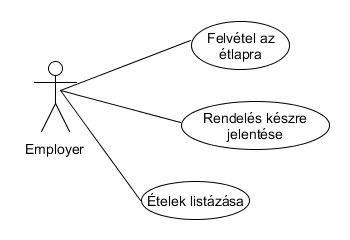
\includegraphics[width=8cm]{uml/UseCase.png}
	\caption{Felhasználói esetdiagram}
\end{figure}

\section{Tervezés}
\subsection{Programszerkezet}Programszerkezet
\begin{itemize}
	\item A programot MVVM architektúrával valósítjuk meg.
	\item A feladathoz a programot két projektre osztjuk. Egy a Order.Persistence, mely
	az adatbázisát és a WebAPI-nak átadott típusait kezeli.
	\item A másik projekt az Order.WPF felelős az app futtatásáért, illetve a funkcióiért.
	Itt találhatóak a View-ViewModel párok, melyekkel megvalósítjuk a különböző oldalakat.
\end{itemize}
\begin{figure}[h]
	\centering
		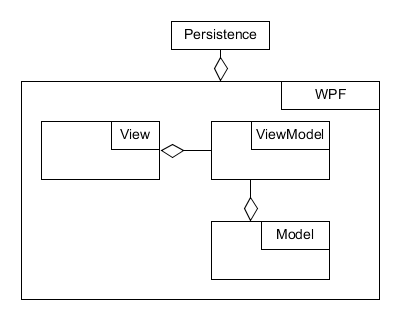
\includegraphics[width=8cm]{uml/WpfBase.png}
	\caption{A WPF app és a perzisztencia szerkezete}
\end{figure}
\newpage
\thispagestyle{empty}
\begin{center}
	\colorbox{lightgray}{{\large B1V655} \hspace{3cm} {\large Webes alkalmazások fejlesztése 2. beadandó} \hspace{5cm} \thepage}
\end{center}

\subsection{Perzisztencia} 
\begin{figure}[h]
	\centering
	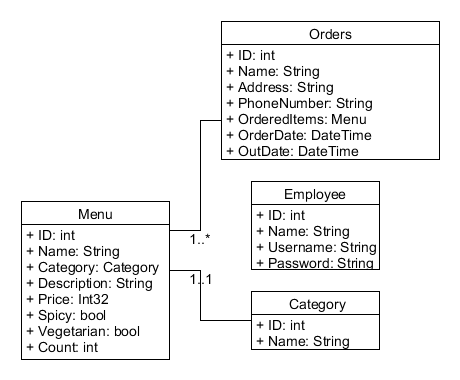
\includegraphics[width=8cm]{uml/Database.png}
	\caption{Az adatbázis kapcsolatok, és táblák}
\end{figure}

\subsection{WPF alkalmazás}
\begin{itemize}
	\item WPF alkalmazás MVVM architektúrában megvalósítva
	\item Model, mely a szerver oldali hívásokat végzi
	\item Szükséges nézetek:
	\begin{itemize}
		\item Login - Bejelentkezés
		\item Menu - Főmenü
		\item AddNewMenuItem - Új étel felvétele az étlapra
		\item Orders - A megrendelések listázása, azok lezárása
	\end{itemize}
	\item Minden nézethez tartozik egy ViewModel
\end{itemize}
		
\subsection{WebAPI}
\begin{itemize}
	\item api/Account/\{username\}/\{password\}:\\[0.1cm]
	HttpGet - Bejelentkezés
	\item api/Account/Logout:\\[0.1cm]
	HttpGet - Kijelentkezés
	\item api/Menu\\[0.1cm]
	HttpPost - Új étel felvétele a Menüre
	\item api/Category/CategoryList\\[0.1cm]
	HttpGet - A kategóriák listázásához szükséges lekérés
	\item api/Orders/OrdersList\\[0.1cm]
	HttpGet - A megrendelések listázásához szükséges lekérés
	\item api/Orders\\[0.1cm]
	HttpPost - Megrendelés készre jelentése.
\end{itemize}

\newpage
\thispagestyle{empty}
\begin{center}
	\colorbox{lightgray}{{\large B1V655} \hspace{3cm} {\large Webes alkalmazások fejlesztése 1. beadandó} \hspace{5cm} \thepage}
\end{center}

\begin{figure}[h]
	\centering
	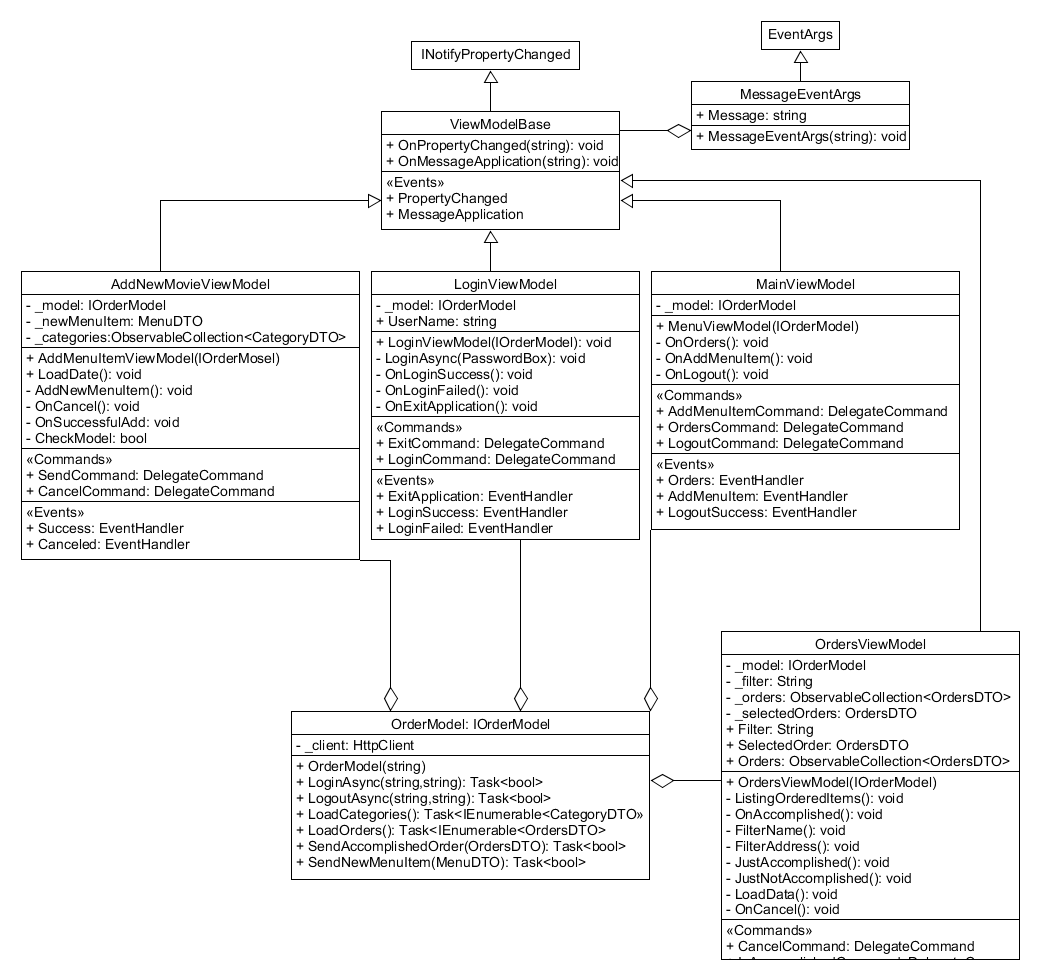
\includegraphics[width=16cm]{uml/ClassDiagram.png}
	\caption{WPF alkalmazás osztálydiagramja}
\end{figure}

\section{Tesztelés}
A webszolgáltatás tesztelése Unit teszteken keresztül történt, egy memóriában létrehozott adatbázis használatával.
\begin{itemize}
\item\textit{GetOrdersTest:} Megrendelések lekérdezése.
\item\textit{GetCategoryTest:} Kategóriák lekérdezése.
\item\textit{AddNewMenuItem:} Új étel hozzáadásának tesztelése.
\item\textit{IsAccompliched:} Készre jelentés tesztelése. 
\end{itemize}
\end{document}